\documentclass[aspectratio=169
  , xcolor={svgnames} 
  , hyperref={ colorlinks,citecolor=DeepPink4
             , linkcolor=DarkRed,urlcolor=DarkBlue}
  , russian
  ]{beamer}
\usetheme{CambridgeUS}
\beamertemplatenavigationsymbolsempty % remove navigation bar
\setbeamertemplate{headline}{}

\makeatletter
\@ifclassloaded{beamer}{
  % get rid of header navigation bar
  \setbeamertemplate{headline}{}
  % get rid of bottom navigation symbols
  \setbeamertemplate{navigation symbols}{}
  % get rid of footer
  %\setbeamertemplate{footline}{}
}
{}
\makeatother
%%%%%%%%%%%%%%%%%%%%%%%%%%%%%%%%%%%%%%%%%%%%%
\usepackage{fontawesome}
% \newfontfamily{\FA}{Font Awesome 5 Free} % some glyphs missing
\expandafter\def\csname faicon@facebook\endcsname{{\FA\symbol{"F09A}}}
\def\faQuestionSign{{\FA\symbol{"F059}}}
\def\faQuestion{{\FA\symbol{"F128}}}
\def\faExclamation{{\FA\symbol{"F12A}}}
\def\faUploadAlt{{\FA\symbol{"F093}}}
\def\faLemon{{\FA\symbol{"F094}}}
\def\faPhone{{\FA\symbol{"F095}}}
\def\faCheckEmpty{{\FA\symbol{"F096}}}
\def\faBookmarkEmpty{{\FA\symbol{"F097}}}

\newcommand{\faGood}{\textcolor{ForestGreen}{\faThumbsUp}}
\newcommand{\faBad}{\textcolor{red}{\faThumbsODown}}
\newcommand{\faWrong}{\textcolor{red}{\faTimes}}
\newcommand{\faMaybe}{\textcolor{blue}{\faQuestion}}
\newcommand{\faCheckGreen}{\textcolor{ForestGreen}{\faCheck}}
%%%%%%%%%%%%%%%%%%%%%%%%%%%%%%%%%%%%%%%%%%%%%

\usepackage{fontspec}
\usepackage{xunicode}
\usepackage{xltxtra}
\usepackage{xecyr}
\usepackage{hyperref}

\setmainfont[
 Ligatures=TeX,
 Extension=.otf,
 BoldFont=cmunbx,
 ItalicFont=cmunti,
 BoldItalicFont=cmunbi,
% Scale = 1.1
]{cmunrm}
\setsansfont[
 Ligatures=TeX,
 Extension=.otf,
 BoldFont=cmunsx,
 ItalicFont=cmunsi,
%  Scale = 1.2
]{cmunss}
%\setmainfont[Mapping=tex-text]{DejaVu Serif}
%\setsansfont[Mapping=tex-text]{DejaVu Sans}
%\setmonofont{Fira Code}[Contextuals=AlternateOff]
\setmonofont{Fira Code}[Contextuals=Alternate,Scale=0.9]
\newfontfamily{\myfiracode}[Scale=1.5,Contextuals=Alternate]{Fira Code}
%\setmonofont[Scale=0.9,BoldFont={Inconsolata Bold}]{Inconsolata}

\usepackage{polyglossia}
\setmainlanguage{russian}
\setotherlanguage{english}


%\newfontfamily\dejaVuSansMono{DejaVu Sans Mono}
% https://github.com/vjpr/monaco-bold/raw/master/MonacoB/MonacoB.otf
%\newfontfamily\monacoB{MonacoB}
%%%%%%%%%%%%%%%%%%%%%%%%%%%%%%%%%%%%%%%%%%%%%%%5
\usepackage{soul} % for \st that strikes through
\usepackage[normalem]{ulem} % \sout

\usepackage{stmaryrd}
\newcommand{\sem}[1]{\ensuremath{\llbracket #1\rrbracket}}


\usepackage{listings}
%\lstdefinestyle{style1}{
%  language=haskell,
%  numbers=left,
%  stepnumber=1,
%  numbersep=10pt,
%  tabsize=4,
%  showspaces=false,
%  showstringspaces=false
%}
%\lstdefinestyle{hsstyle1}
%{ language=haskell
%%          , basicstyle=\monacoB
%         , deletekeywords={Int,Float,String,List,Void}
%         , breaklines=true
%         , columns=fullflexible
%         , commentstyle=\color{ForestGreen}
%         , escapeinside=§§
%         , escapebegin=\begin{russian}\commentfont
%         , escapeend=\end{russian}
%         , commentstyle=\color{ForestGreen}
%         , escapeinside=§§
%         , escapebegin=\begin{russian}\color{ForestGreen}
%         , escapeend=\end{russian}
%         , mathescape=true
%%          , backgroundcolor = \color{MyBackground}
%}
%
%\newcommand{\inline}[1]{\lstinline{haskell}{#1}}
%\def\hsinline{\mintinline{haskell}}
%\def\inline{\hsinline}
%
%\lstnewenvironment{hslisting} {
%    \lstset { style={hsstyle1} }
%  }
%  {}
%  
%%%%%%%%%%%%%%%%%%%%%%%%%%%%%%%%%%%%%%%%%%%%%%%%%%%%%%%%%%%  
%%\setmainfont[
%% Ligatures=TeX,
%% Extension=.otf,
%% BoldFont=cmunbx,
%% ItalicFont=cmunti,
%% BoldItalicFont=cmunbi,
%%]{cmunrm}
%%% С засечками (для заголовков)
%%\setsansfont[
%% Ligatures=TeX,
%% Extension=.otf,
%% BoldFont=cmunsx,
%% ItalicFont=cmunsi,
%%]{cmunss}
%% \setmonofont[Scale=0.6]{Monaco}
%
%\usefonttheme{professionalfonts}
%\usepackage{times}
\usepackage{tikz}
\usetikzlibrary{cd}
\usepackage{tikz-cd}
\usepackage{caption}
\usepackage{subcaption}

%\renewtheorem{definition}{برهان}[chapter]
%%\DeclareMathOperator{->}{\rightarrow}
%\newcommand\iso{\ensuremath{\cong}}
%\usepackage{verbatim}
%\usepackage{graphicx}
%\usetikzlibrary{arrows,shapes}

%\usepackage{amsmath}
%\usepackage{amsfonts}
\usepackage{scalerel}
\DeclareMathOperator*{\myvee}{\scalerel*{\vee}{\sum}}
\DeclareMathOperator*{\mywedge}{\scalerel*{\wedge}{\sum}}

%
%\usepackage{tabulary}
%
%% sudo aptget install ttf-mscorefonts-installer
%%\setmainfont{Times New Roman}
%%\setsansfont[Mapping=tex-text]{DejaVu Sans}
%
%%\setmonofont[Scale=1.0,
%%    BoldFont=lmmonolt10-bold.otf,
%%    ItalicFont=lmmono10-italic.otf,
%%    BoldItalicFont=lmmonoproplt10-boldoblique.otf
%%]{lmmono9-regular.otf}
%
\usepackage[cache=true]{minted}
\usemintedstyle{perldoc}

\def\hsinline{\mintinline{haskell}}
\def\mlinline{\mintinline{ocaml}}
% color options
\definecolor{YellowGreen} {HTML}{B5C28C}
\definecolor{ForestGreen} {HTML}{009B55}
\definecolor{MyBackground}{HTML}{F0EDAA}



\institute{матмех СПбГУ}

\addtobeamertemplate{title page}{}{
  \begin{center}{\tiny Дата сборки: \today}\end{center}
}


% \usepackage{tabularx}  % for 'tabularx' environment
% \usepackage{ragged2e} % for \Centering macro
% \newcolumntype{C}{>{\Centering\arraybackslash}X}m
% sudo aptget install ttf-mscorefonts-installer

%\setmainfont{Times New Roman}
%\setsansfont{CMU Sans Serif}


\usepackage{tabulary}
\usepackage{verbatim}
\newcommand{\term}[2]{\textit{#1} (#2)}

\usepackage[cache=true]{minted}
\usepackage{amsthm}

\newtheorem{remark}{\textbf{Замечание}}[section]
\newtheorem{hint}{\textbf{Указание разработчикам}}[section]

\newtheoremstyle{exerciseStyle1}
{}                % Space above
{}                % Space below
{}                % Theorem body font % (default is "\upshape")
{}                % Indent amount
{\bfseries}       % Theorem head font % (default is \mdseries)
{.}               % Punctuation after theorem head % default: no punctuation
{ }               % Space after theorem head
{}                % Theorem head spec
\theoremstyle{exerciseStyle1}
\newtheorem{exercise}{\textbf{Упражнение}}[section]


\deftranslation[to=russian]{Theorem}{Теорема}
\deftranslation[to=russian]{theorem}{теорема}

\usepackage{tikz}
\usetikzlibrary{trees}
\usepackage{subcaption}

%%%%%%%%%%%%%%%%%%
\makeatletter
\newenvironment{tabminted}{%
  \let\FV@ListVSpace\relax  
  \minted
}{%
  \endminted
  \unskip   
  \aftergroup\@tabmintedend
}
\newcommand*{\tabminted@finalstrut}[1]{%
  \ifdim\prevdepth>0pt
    \ifdim\dp#1>\prevdepth
      \vskip\dimexpr(\dp#1)-\prevdepth\relax
    \fi
  \else
    \vskip\dimexpr(\dp#1)\relax
  \fi
}
\newcommand*{\@tabmintedend}{%
  \let\@finalstrut\tabminted@finalstrut
}
\renewcommand{\cite}[1]{}
\makeatother


%%%%%%%%%%%%%%%%%%%%%5
\title[Retrofitting Parallelism onto OCaml]{Retrofitting Parallelism onto OCaml}
\subtitle{Переоснащение параллелизма для OCaml}
\author{Косарев Дмитрий }

\institute{матмех СПбГУ}

\date{\today}
 
\AtBeginSection[]
{
  \begin{frame}<beamer>%[allowframebreaks]
    \frametitle{Оглавление}
    \tableofcontents[currentsection,currentsubsection]
  \end{frame}
}

\AtBeginSubsection[]
{
   \begin{frame}
        \frametitle{Оглавление}
        \tableofcontents[currentsection,currentsubsection]
   \end{frame}
}

\newcommand{\verbatimfont}[1]{\def\verbatim@font{#1}}
\setcounter{tocdepth}{1}  % part,chapters,sections
\setcounter{tocdepth}{2}  % part,chapters,sections,subsections
%\newcommand\chap[1]{
%  \chapter*{#1}
%  \addcontentsline{toc}{chapter}{#1}
%}

\usepackage{verbatimbox}

\begin{document}
\maketitle

% For every picture that defines or uses external nodes, you'll have to
% apply the 'remember picture' style. To avoid some typing, we'll apply
% the style to all pictures.
\tikzstyle{every picture}+=[remember picture] 

% By default all math in TikZ nodes are set in inline mode. Change this to
% displaystyle so that we don't get small fractions.
\everymath{\displaystyle}

% Uncomment these lines for an automatically generated outline.
\begin{frame}{Оглавление}
  \tableofcontents
\end{frame}

\begin{frame}{Введение}
В мире много расширений языка ML для поддержки параллелизма (Manticore, MultiMLton)
\vspace{1cm}

Целью этой работы является 
\begin{itemize}
  \item Переоснастить GC языка OCaml
  \item Предварительно посмотрев на Go, .NET CLR, Haskell
\end{itemize}
\end{frame}

\begin{frame}{Введение}
Вообще, concurrensy/parallelism обычно нужен для трех типов задач:

\begin{itemize}
\item Parallelism on shared-memory multiprocessors
\item Чередование ввода-вывода и вычислений (когда нить блокируется, ожидая чтения по сети, а остальные могут работать)
\item  Стиль программирования c корутинами% "coroutine" 
\end{itemize}\vspace{1cm}

\href{https://flyingfrogblog.blogspot.com/2017/04/xavier-leroys-standard-lecture-on.html}{Xavier Leroy's "standard lecture on threads" }
\end{frame}

\section{Требования}
\begin{frame}[fragile]{Performance backwards compatibility}
\begin{itemize}
  \item  Выделение памяти должно быть быстрым
  \item Большиноство объектов иммутабельны
  \item Для изменяемых объектов
  \begin{itemize}
  \item инициализация без барьера
  \item чтение без барьера
  \item присваивание -- с барьером
  \end{itemize}
  \item Мажорная куча
  \begin{itemize}
  \item  incremental, non-moving, mark-and-sweep collector
  \item уплотнение опционально
  \end{itemize}
  \item Хочется иметь один рантайм, а не два, как в Haskell
\end{itemize}

\note{Выделение памяти -- просто увеличение указателя минорной кучи

Мажорная куча позволяет писать latency sensitive приложения, например сетевые
}
\end{frame}

\begin{frame}{ Feature backwards compatibility}
\begin{itemize}
  \item Хотим при добавлении параллелизма сломать как можно меньше существующего кода на OCaml кода 
  \item  Bounding Data Races in Space and Time (PLDI 2018)
  -- модель памяти с разумным оверхэдом

  \item weak references, finalisers, ephemerons, lazy values
  \item OCaml’s C API e
  \begin{itemize}
\item  чтение любого объекта OCaml, мутабельного или нет, из API языка C проиходит без барьера чтения
  \end{itemize}
\item Хотим выдержать баланс между сложностью C API и упущенными возможностями по оптимизации
\end{itemize}

\end{frame}

\begin{frame}{Требования}
\begin{itemize}
  \item Корректные последовательные программы не ломаются при параллельном исполнении 
  \item Производительность в последовательном и параллельном runtime примерно такая же. То же про паузы из-за GC
 
  \item Параллельные программы 
  \begin{itemize}
  \item в начале минимизируют паузы
  \item затем оптимизируют производительность
  \end{itemize}

\end{itemize}
\note{
\begin{itemize}
\item That is, a well-typed
  serial program remains well-typed in the parallel extension, and the semantics of such a   program remains the same on the serial and parallel runtimes.
\item 
\item   We order the sub goals this way since minimising pause times
  in the GC is much harder than achieving good throughput. We believe that once the pause  times are optimised for, optimising for throughput is easier, but the vice versa is much harder  
\end{itemize}
}
\end{frame}

\begin{comment}
\begin{frame}{Про мажорную кучу. Может перенсти ниже?}
\begin{itemize}
  \item We develop a generational garbage collector with two generations where the old generation
  (major heap) is shared between all of the mutators and is collected with a non-moving, mostly-
  concurrent, mark-and-sweep collector modelled on VCGC [Huelsbergen and Winterbottom 1998].
  VCGC avoids having explicit phase transitions between marking and sweeping, which is the
  traditional source of bugs in concurrent collector designs. For programs that do not use weak
  references or ephemerons, the mutator and the GC threads need to synchronize only once per cycle
  to agree that the current cycle is done. This minimizes the pause times. The major heap allocator is
  based on the Streamflow [Schneider et al. 2006] design, which uses size-segmented thread-local
  pages. This has been shown to have good multicore behaviour and fragmentation performance
\end{itemize}
\end{frame}

\begin{frame}{Может перенсти ниже?}
The original quasi-real-time collector design by [Doligez and Leroy 1993] maintains the invariant
that there are no pointers from major to minor heaps. Thus, storing a pointer to a private object into
the shared major heap causes the private object and all objects reachable from it to be promoted
to the shared heap en masse. Unfortunately, this eagerly promotes many objects that were never
really shared: just because an object is pointed to by a shared object does not mean another thread
is actually going to attempt to access it. A good example is a shared work-stealing queue, where
stealing is a rare operation. It would be unwise to promote all the work to the major heap.
\end{frame}
\end{comment}


\begin{frame}{Два новых сборщика мусора для младшего поколения}
\begin{itemize}
  \item Concurrent minor collector с приватными младшими поколениями
  \begin{itemize}
  \item Объекты переезжают в старшее поколение, если из старшего поголения они достижимы, т.е. независимо от того, читали ли их из других потоков, или нет
  \item Операция переноса объекта в общую память станоиться сложнее, но вызывается реже
  \item Дизайн требует, чтобы чтение было точкой безопасности (safe point), где можно провести сборку мусора
\note {
Consider the case of two
mutators both of which are trying to read an object in the minor heap of the other mutator. In
order to make progress, the mutators will have to service promotion requests that they receive
while waiting for their request to be satisfied. Recall that stock OCaml does not use read barriers
and the C API also works under this assumption. By making the reads safe points, it is likely that
every user of the C API will need to update their code to conform with the new semantics. This
conflicts with our first requirement.
}

  \end{itemize}
  \item  Stop-the-world parallel minor collector
  \begin{itemize}
\item  Все должны синхронизировать перед сборкой мусора, ценой того, что  возможны б\'ольшие паузы 
\item  Способы доступа к памяти те же, т.е. не над изменять C API
\note{
\item the stop-the-world
minor collector outperforms the concurrent minor collector in almost all circumstances, even as
we cranked up (сделали максимальным) the number of cores.
}
  \end{itemize}
\end{itemize}
\end{frame}

\begin{frame}[fragile]{Достижения}
\begin{itemize}
  \item Дизайн mostly-concurrent, non-moving, mark-and-sweep GC для старшего поколения с минимизацией пауз
  \item Два дизайна сборщиков мусора для младшего поколения 
  \begin{itemize}
  \item конкуретный, который минимизирует паузы ценой изменений  C API 
  \item  stop-the-world parallel collector, сохраняющий обратную совместимости с C API
  \end{itemize}
  
  \item Расширения сборщиков мусора для продвинутых возможностей языка: ленивые значения, слабые ссылки и  ephemerons. 
  
  
  \item Fibers -- parallel, language level lightweight threads implemented as runtime managed stack segments. По аналогии с GHC и Go-рутинами

  \item Эксперименты
%  \begin{itemize}
%  \item serial programs retain their performance
%   profile on the new collectors,
%   \item parallel programs achieve good multicore scalability
%    while preserving low pause times with increasing number of cores.
%  \end{itemize}
\end{itemize}
\note{
\begin{itemize}
\item \item 
\item Our novel design minimizes
  the number of global synchronizations necessary for collecting a deeply nested hierarchy of
  ephemerons. This design has been verified in the SPIN model checker.
  
\item   The implementation of fibers is similar to
  lightweight threads in Haskell GHC and Goroutines in the Go language. While the details
  of the language support for fibers is beyond the scope of the paper, we describe the subtle
  interaction of our concurrent GC algorithm with fibers.
\end{itemize}
}
\end{frame}

\begin{frame}[fragile]{Обзор памяти OCaml}

\begin{figure}[ht]
\begin{subfigure}{.49\textwidth}
Uniform представление в памяти $\Leftrightarrow$ все значения одного размера $\Rightarrow$ позволено иметь только один скомпилированный вариант для каждой полиморфной функции [Appel 1990].
\vspace{1cm}


Все значения 32/64-битные и либо
\begin{itemize}
\item числа (младший бит 1)
\item указатели
\end{itemize}

У указателей младшие биты всегда 0, так как значения выровнены в памяти
\end{subfigure}
\hspace{.5cm}
\begin{subfigure}{.39\textwidth}

Каждый объект OCaml имеет заголовок, где есть длин, тип и пара битов для цветов, которые используются во время GC \vspace{1cm}

Два поколения
\begin{itemize}
\item Старшее -- major heap
\item Младшее -- minor heap
\end{itemize}

"Корни" локальные и глобальные, remembered set и т.д.

Аллокаторы
\begin{itemize}
\item Младшее -- bump pointer
\item Старшее -- разные
\end{itemize}
\end{subfigure}
\end{figure}
\note{
The least significant bit (LSB) is used to distinguish integers and pointers: since
all allocations are word-aligned, the LSB of pointers is guaranteed to be zero, whereas integers are
encoded by left-shifting the integer value by one, and setting the LSB to one.
}
\end{frame}
\begin{comment}
\begin{frame}{}
Младшее поколение
\begin{itemize}
  \item Сборка мусора при переполнении с копированием в главную кучу
\end{itemize}
The minor collection proceeds by first promoting all the roots (globals, local roots
registered in C calls, registers, the remembered set of inter-generational pointers from the major to
the minor heap, and the program stack) that point to the minor heap to the major heap, and then
transitively promoting all the referenced objects. All references from live objects to objects in the
minor heap are updated to point at the new location, including references from the major heap to
the minor heap (recorded in the remembered set), and the old minor heap is then reused in the
next cycle. The copying collector only needs to touch the live objects. Given that the survival rate
in the minor collection is low, a copying collector minimizes pause times.
\end{frame}
\end{comment}

\section{Старшее поколение (major heap)}

\begin{comment}
content

\begin{frame}[fragile]{Старшее поколение в текущем OCaml УДАЛИТЬ} 
The major heap contains objects which have survived a minor collection (as well as objects above
a certain size, which are allocated there directly). Instead of a bump-pointer algorithm, allocation
in the major heap uses a more sophisticated allocator, which differs between stock and Multicore
OCaml. The major GC is incremental, except for an optional stop-the-world compaction phase.

\end{frame}
\end{comment}


\begin{frame}{
Старшее поколение в \only<1>{однопоточном}\only<2>{параллельном} OCaml
}
Однопоточный OCaml
\begin{enumerate}
  \item \textit{Mark-and-sweep} %Collection is divided into two phases: marking determines which allocations  are still in use, and sweeping collects those that are not and makes them available for reuse.
  \item \textit{Incremental} -- сборка мусора выполняется по частям, которые называются \textit{slices}
  \item \textit{Compaction} -- опциональная фаза
  %\item   \textit{Non-moving} %Once allocated in the major heap, objects remain at the same address until collected.
\end{enumerate}\vspace{1cm}
\pause
Параллельный OCaml 
\begin{enumerate}
  \item \textit{Mark-and-sweep} 
  \item \textit{Incremental}
  \item \sout{\textit{Compaction}} Non-moving
  \item ещё и параллелен: 
  \emph{домены} выполняются в системных потоках и одном адресном пространстве %\vspace{1cm}
\end{enumerate}

\note{
\begin{itemize}
\item \textit{Incremental} Rather than stopping the program for the whole duration of GC (which would cause
  a pause bounded in length only by the size of memory), the OCaml major collector pauses  the program in many small slices.
\end{itemize}

Multicore OCaml’s collector retains these properties, and is also parallel: the virtual machine
contains a number of domains, each running as a separate system thread in the same address space. Domains can be dynamically created and brought down.

A garbage collector uses a large amount of shared mutable state, as the collector must track how
each byte of memory is being used. The central challenge in writing a multicore garbage collector
is controlling access to this state without introducing too much expensive synchronisation. To
understand this challenge, we first review how this state is used in the stock OCaml collector.
}
\end{frame}

\begin{frame}{Основная проблема}

В GC много изменяемого состояния\vspace{.5cm}

\begin{block}{Основная проблема}
Реализовать параллельный сборщик мусора, чтобы не требовалось много синхронизации для работы с изменяемым состоянием.
\end{block}
Были прецеденты...
\end{frame}


\subsection{Цветная раскраска}

\begin{frame}{\sout{Трёх}Четырёхцветная раскраска}
\begin{figure}[ht]
\begin{subfigure}{.49\textwidth}
Dijkstra et al 1978
\begin{enumerate}
\item black
\item gray 
\item white
\item blue --  синие -- не объекты, но свободная память
\end{enumerate}
\end{subfigure}
\begin{subfigure}{.49\textwidth}
\begin{enumerate}
\item marking \item sweeping
\end{enumerate}
Чередуются с пользовательским кодом, который может присваивать и \textit{аллоцировать}
\end{subfigure}
\end{figure}

\end{frame}

\begin{frame}{Marking}

\begin{figure}[ht]
\begin{subfigure}{.49\textwidth}
\begin{itemize}
  \item живые объекты -- черные
  \item найденный мусор -- белые
  \item граница -- серые
\end{itemize}
Начинается с корней
\begin{itemize}
\item Неинкрементально -- регистры и стек
\item Инкрементально -- глобальные корни (их может быть много, поэтому инкрементальность $\Rightarrow$ меньше пауз)
\end{itemize}
\end{subfigure}
\begin{subfigure}{.49\textwidth}
Маркировка превращает белые объекты в серые  и кладет их в стек замаркированных (mark stack) \vspace{.5cm}

После корней маркируются объекты со стека и достижимые из них \vspace{.5cm}

Всё заканчивается, когда стек пуст $\Leftrightarrow$ нет больше серых объектов

%After the roots are marked, marking is continued by popping the mark stack, marking the
%children of the object popped, and then marking the object black. This process is repeated until the
%mark stack becomes empty, meaning that there are no more gray objects.

\end{subfigure}
\end{figure}
\end{frame}

\begin{frame}{Sweeping --- стандартно}
После окончания маркировки
\begin{itemize}
\item объекты, которые всё ещё используются --- черные 
\item мусор --- белый
\end{itemize}

Sweeping --- один инкрементальный обход кучи, преобразующий 
\begin{itemize}
\item черные $\Rightarrow$ в белые
\item белые $\Rightarrow$ в синие
\end{itemize}
 
%, to indicate that their storage is now free to be used for future allocations.

\end{frame}

\begin{frame}{Присваивание}
При присваивании в программе используется \textit{ write barrier}. \\

Во время маркировки старые значения тоже обрабатываются: белые перекрашиваются в серые

\begin{block}{Инвариант (snapshot-at-the-beginning)}
Любой объект, достижимый в начале стадии маркировки рано или поздно покрасится.
%that every object reachable at the start of marking eventually gets marked
\end{block}

%During the
%mark phase of the GC, the write barrier loads the object pointed to by the old value of the field, and
%if it is white, grays it and adds it to the mark stack. This preserves the invariant  (the \textit{snapshot-at-the-beginning property}).
\note {
The write barrier also keeps track of the inter-generational pointers from major to minor heap
in a remembered set, which is used as a root for the minor collection. (See section 4).
}
\end{frame}

\begin{frame}{Свежие выделения памяти}
Свежие выделения памяти надо раскрашивать, чтобы они сразу же не собрались GC\vspace{1cm}

В время маркировки -- в черный\vspace{1cm}

Во время удаления мусора (sweeping) -- зависит дошло ли до них дело
\begin{itemize}
\item если тут уже удаляли -- то в белый 
\item если нет, то в черный, а потом GC покарасит в белый, если надо будет
\end{itemize}
\end{frame}

\begin{frame}{Можно раскрашивать по-разному}
OCaml делает так:
\begin{itemize}
\item Делает серыми старые значения во время присваивания (\textit{deletion barrier} [Yuasa 1990])
\item Красит корни \emph{до} всего остального (\textit{black mutator})
\end{itemize}
И из-за этого
\begin{itemize}
\item[+] Ограниченное количество работы на цикл GC
\item [---] Некоторые объекты соберутся позже чем могли
\end{itemize}
\vspace{.5cm}

Детали искать в Vechev et al. [2005] или Jones et al. [2011] \vspace{.5cm}

Но они ортогональны многопоточному GC
%for further discussion of these
%details. We will not discuss them further here, as the trade-offs involved are largely independent of
%the switch from a single-threaded to a multi-threaded GC.

\end{frame}

\begin{frame}{Изменяемое состояние, вовлеченное в дизайн}
Перечислим:
\begin{itemize}
  \item Между marking и sweeping: цвета, смысл которых меняется между фазами%the object colours, whose meaning changes between phases)
  \item Между присваиванием и marking: write barrier порождает новые серые объекты %supplies new gray objects to the collector)
  \item Между выделением объектов и sweeping: нужно определять фазу и  позицию, а также совместно управлять информацией о свободной памяти
  %allocation must determine the phase of the collector and position
  %of sweeping, as well as coordinating with the sweeper to manage free memory).
\end{itemize}
\vspace{1cm}
Для однопоточного сборщика мусора это вполне нормально, но для много поточного реализовать всё правильно -- сложно (были прецеденты)
\end{frame}

\subsection{Многопоточный сборщик мусора в OCaml} 

\begin{frame}{Многопоточный GC OCaml: долой изменяемое состояние}

Хотим по максимуму \textbf{избавиться от изменяемого состояния}
\vspace{1cm}

Вначале сократим разделенное состояние \textit{между потоками и GC}
\begin{itemize}
  \item не используем серый цвет
  \item у каждого домена свой стек серых объектов
  %each domain maintains its own stack of gray objects, and 
  \item если барьер чтения хочет сделать объект серым, то он кладет его на стект домена
 % ds to gray  an object it marks it and adds it to the local domain’s gray stack.
  \item в одном домене GC и полезный код чередуются -- синхронизация не нужна.
\end{itemize}
\end{frame}

\begin{frame}{Избегаем изменяемого состояния между marking и sweeping}
\begin{itemize}
  \item Частично переиспользуем Very Concurrent Garbage  Collector (VCGC)\cite{VCGC}
  \item Там \textit{нет} отдельных фаз  marking и sweeping, а также там 2 цвета объектов
  \item У нас будет как бы  4 состояния у памяти
  \begin{itemize}
  \item для занятой -- Marked, Unmarked и Garbage
  \item для свободной -- Free
  \end{itemize}
  \item Процесс перекраски такой
\begin{itemize}
  \item marking:  \texttt{Unmarked}  $\Rightarrow$ \texttt{Marked}
  \item sweeping:  \texttt{Garbage} $\Rightarrow$ \texttt{Free} 
\end{itemize}
\item Множества на которых, работают merking и sweeping, не пересекаются -- синхронизация не нужна
\item Только что выделенные -- \texttt{Marked} -- чтобы не собрались прям сразу
\item Для определения цвета не нужна синхронизация
  \end{itemize}
\end{frame}

\begin{frame}[fragile]{Разделение состояния между доменами}
которые делают одну и ту же фазу сборки мусора
\begin{itemize}
  \item Сделаем  marking \textit{idempotent} 
  \item А sweeping  \textit{disjoint}
\end{itemize}\vspace{.5cm}

Разные домены могут одновременно замаркировать объект, и мы этого не избегаем\\

Мы разрешаем одному и тому же объекту быть замаркированным дважды, зная что это даст тот же результат. Это гораздо дешевле, чем синхронизация каждого объекта\\

%Multiple domains may attempt to mark the same object at the same time, and we make
%no attempt to avoid this. Instead, we allow the occasional object to be marked twice, knowing
%that this gives the same result as marking once. Allowing for this possibility is much cheaper than
%synchronising each access to an object by the collector.

Sweeping не идемпотентен и мы собираем в домене только ту память, которую это домен выделил 
%is not idempotent. Instead, we ensure that the areas swept by different domains are
%disjoint: each domain sweeps only the memory that it allocated, keeping the interaction between
%sweeping and allocation local to a domain
\end{frame}

\begin{frame}{}
Единственная точка синхронизации -- в конце цикла сборки.

\begin{itemize}
  \item Когда у всех маркировочные стеки пусты (только недостижимые объекты помечены \texttt{Unmarked})
  \item и sweeping закончен, т.е. больше нет \texttt{Garbage} -- они все превратились во \texttt{Free}
  \item все домены останавливаются  (deletion barrier) и переставляются биты
  
  \begin{itemize}
  \item Marked $\Rightarrow$ Unmarked
  \item those for Unmarked  $\Rightarrow$  Garbage
  \item  Garbage  $\Rightarrow$  Marked
  \end{itemize}
  \item Это делается для всех доменов, но это константное количество работы, надо только выбирать правильный момент, когда это делать

%This must be done with all domains stopped, but is a small,
%constant amount of work, for which the only difficulty is deciding when it should happen.
\end{itemize}
\end{frame}



\begin{frame}[fragile]{Детектируем окончание сборки мусора}
\begin{figure}[ht]
\begin{subfigure}{.49\textwidth}
\begin{minted}[escapeinside=||]{python}
def majorSlice(budget):
  budget = sweepSlice(budget)
  budget = markSlice(budget)
  if ( budget && |!|dlMarkingDone ):
    dlMarkingDone = 1
    atomic:
      gNumDomsToMark--
  if (gNumDomsToMark == 0):
    runOnAllDoms(cycleHeap)
\end{minted}
\end{subfigure}
\begin{subfigure}{.49\textwidth}
deletion barrier $\wedge$  new objects сразу момечаются как \texttt{Marked},  $\Rightarrow$ количество работы в каждом цикле конечное ( свойство snapshot-at-the-beginning).\vspace{.5cm}

g $\equiv$ global\\
dl $\equiv$ domain-local \vspace{.5cm}

Когда стек замаркированного очищается -- декрементим домены
\end{subfigure}
\end{figure}
\end{frame}



\begin{frame}[fragile]{Heap cycling}
\begin{figure}[ht]
\begin{subfigure}{.49\textwidth}
\begin{minted}[escapeinside=||]{python}
def cycleHeap ():
  barrier :
    /* run only by last domain to 
       reach barrier */
    newc.Unmarked = gColours.Marked
    newc.Garbage = gColours.Unmarked
    newc.Marked = gColours.Garbage
    newc.Free = gColours.Free
    gColours = newc
    gNumDomsToMark = gNumDoms
  dlMarkingDone = 0
  markNonIncrementalRoots ()
\end{minted}
\end{subfigure}
\begin{subfigure}{.49\textwidth}
Последний домен под барьером только переделывает смысл цветов и настраивает количество доменов на следующий цикл, т.е. делает очень мало $\Rightarrow$ мало пауз
\vspace{1cm}

Свеже созданные домены не добаляются в gNumDomsToMark, потому что там собирать на этом цикле нечего
\end{subfigure}
\end{figure}
\end{frame}

\subsection{Allocator}

\begin{frame}{Аллокатор для старшего поколения}
\begin{figure}[ht]
\begin{subfigure}{.95\textwidth}
В OCaml все выделенные объекты уже инициализированы.\vspace{.5cm}

Цель: цена выделения должна быть пропорциональна цене инициализации\\
т.е. мелкие объекты должны выделяться быстро, а большие могут медленнее.\\

Бывают разные стратегии:
\begin{itemize}
\item first-fit
\item next-fit
\item best-fit (в текущем OCaml)
\end{itemize}
Все однопоточные\vspace{.5cm}

Нельзя перенести в многопоточный режим, потому что lock будет слишком дорогой
\end{subfigure}
\begin{subfigure}{.49\textwidth}

\end{subfigure}
\end{figure}
\end{frame}



\begin{frame}{На основе Streamflow\cite{streamflow}}
\begin{itemize}
  \item Для \textit{мелких }аллокаций (<128 words) -- локальный для домена, size-segmented список страниц 
  %Each page of 4K words is carved into equal-sized slots, with size
  %classes chosen so that there is less than 10\% wasted space.
  \item Для \textit{больших} аллокаций используются системные malloc/free.
  \item Локальные для домена список больших блоков
  \item При смерти домена добавляются в глобальный список (защищенный мьютексом) осиротевших (orphaned) блоков
  % потому что к ним могу стучаться из других потоков.
\end{itemize}
\vspace{.5cm}

Streamflow использует BiBoP~\cite{bibop}, чтобы следить, какие слоты свободны, котором не нужны дополнительные заголовки. Но в OCaml заголовки уже есть, так что используются они
\end{frame}



\begin{frame}{Выделение в старшем поколении}
Когда нужно что-то выделить в мажорной куче
\begin{enumerate}
\item Ищется подходящее место в локальном списке страниц подходящего размера
\item Если там нет подходящих, пытается собрать удалить неиспользующиеся
\item Если всё ещё нет слота, то используется одна из глобального списка страниц
\item Если нет, то используется занятая страница, там собирается мусор и ищется слот
\item Если всё не так, то просится новая страница у операционной системы
\end{enumerate}
Итого, большинство аллокаций можно сделать без атомиков и синхронизаций
\end{frame}



\begin{frame}{Safe points}
Позволяют знать, когда можно делать stop-the-world\vspace{.5cm}

Дополняют моменты, когда делается аллокация \vspace{.5cm}

Используется алгоритм, который выбирает точку после определенного числа инструкций\vspace{.5cm}

Они и так присутствуют в однопоточном OCaml

\note{
 These safe points are necessary to avoid deadlocks in
certain situations e.g one domain in a non-allocating loop spin-waiting on an empty queue while all
other domains need a minor collection in order to allocate new items to put on the queue. 
}

\end{frame}



\begin{frame}{Opportunistic work}
\begin{itemize}
  \item \textit{Yielding}. Например, инструкция PAUSE на x86
  \item \textit{Stop-the-world entry waits} Когда stop-the-world GC для младшего поколения создает паузу
\end{itemize}

Ещё можно в другие моменты, но это future work
\end{frame}

\section{Младшее поколение (minor heap)}

\begin{frame}{Особенности младшего поколения}
Много меньше, чем старшее поколение, но тут чаще выделяется/собирается мусор\vspace{1cm}

В отличие от старшего поколения
\begin{itemize}
\item Копирует. Из младшего в старшее
\item Неинкрементальное -- паузы
\end{itemize}

\end{frame}

\begin{frame}{Младшее поколение в однопоточном OCaml}
К "корням" добавляется remembered set -- ссылки из старшего поколения
Не надо ходить по старшему поколению и искать ссылки на младшее\\

Копируется мало: мало объектов и они малы. Поэтому мало пауз\\

Не нужно хитрых аллокаторов, обычный bump-pointer подойдет
\end{frame}

\begin{frame}{Распараллеливание GC младшего поколения}
Это сложнее так, как объекты могут передвигаться в старшее поколение, в то время как используются другим потоком\\

Можно реализовать аккуратно скоординировав мутаторы и GC: храня в общей памяти какие объекты были перемещены\\

Высокая цена: требует синхронизации на любой доступ к памяти\\

Остается два варианта разделения мутатора и GC
\begin{enumerate}
\item В пространстве: запретим доступ в другой домен  и разрешим собирать мусор по-отдельности

\item Во времени: когда младшее поколение заполнено, то все домены останавливаются и параллельно собирают мусор
\end{enumerate}
\end{frame}

\subsection{Конкурентный сборщик младшего поколения с приватными кучами}

\begin{frame}{Конкурентный сборщик младшего поколения с приватными кучами}
У каждого домена 
\begin{itemize}
\item свои приватные кучи
\item свой remembered set
\end{itemize}
%domain-local, private, minor heap arenas, each tracking their
%own remembered set. 

\begin{block}{Инвариант}
Нет указателей между младшими поколениями разных доменов 
(что позволяет собирать мусор независимо)
\end{block}
%We maintain the invariant that there are no pointers between the minor
%heaps of different domains, which permits each of the minor heaps to be independently collected.

Мы разрешаем указатели из общей major кучи в минорную, чтобы не страдать от 
early promotion (так же сделано в multicore GHC [Marlow and Peyton Jones 2011])


\end{frame}

\begin{frame}{Read faults и interrupts}
Read fault происходит когда переходим по указателю из мажорной кучи в минорную кучу другого домена.\\

У каждого домена есть multiple-producer single-consumer queue\\

Отправитель посылает запрос, и ограничивает возможности получателя аллоцировать в минорной куче, чтобы быстрее синхронизироваться
(примерно то же делается со сборками старших куч)\\

Получатель передвигает объект и его транизитивное замыкание в мажорную кучу отправителя\\

Пока отправитель ждет, он обрабатывает запросы пришедшие к нему (чтобы не было deadlock'ов)

\end{frame}

\begin{frame}{Барьер чтения}
\begin{figure}[ht]
\begin{subfigure}{.59\textwidth}
Важно соптимизировать его, потому что его не было в однопоточном OCaml

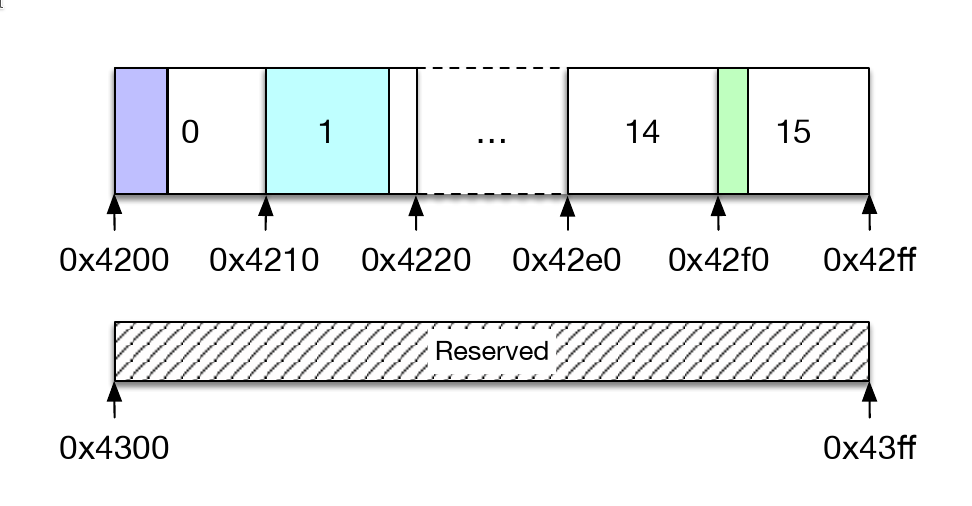
\includegraphics[scale=.35]{img1}
\end{subfigure}
\hspace{.5cm}
\begin{subfigure}{.35\textwidth}
Пример 16битное адресное пространство \texttt{0xPQRS}.\\
R -- домен\\
Значения в минорной куче: PQ=42\\
У чисел S = 1\\ \vspace{0.5cm}

С таким подходом излишне резервируется некоторое количество виртуальной памяти, но это не так уж страшно

\end{subfigure}
\end{figure}
\end{frame}

\begin{frame}[fragile]{}
\begin{figure}[ht]
\begin{subfigure}{.49\textwidth}
Алгоритм (константное число действий)
\begin{minted}[escapeinside=||]{asm}
# ax = value of interest 
# bx = allocation pointer 
xor %bx , %ax
sub 0x0010, %ax
test 0xff01, %ax
# ZF set |$\Rightarrow$| ax in remote minor 
\end{minted}
Инструкция \texttt{test} делает \& и проставляет флаг ZF если результат 0
\end{subfigure}
\begin{subfigure}{.49\textwidth}
Значения бывают 4х классов
\begin{enumerate}
\item Число
\item Указатель в мажорную кучу
\item Указатель в свою минорную кучу
\item Указатель в чужую минорную кучу
\end{enumerate}
\end{subfigure}
\end{figure}
\end{frame}

\begin{frame}[fragile]{Четыре случая (3/4)}
\begin{figure}[ht]
\begin{subfigure}{.3\textwidth}
\begin{minted}[escapeinside=||]{asm}
# low_bit (ax) = 1 
# low_bit (bx) = 0
xor %bx , %ax
# low_bit (ax) = 1
sub 0x0010 , %ax
# low_bit (ax) = 1 
test 0xff01 , %ax
# ZF not set 
\end{minted}
\caption{Case: Integer}
\end{subfigure}
\begin{subfigure}{.3\textwidth}
\begin{minted}[escapeinside=||]{asm}
# PQ (ax)= 0x42 
# PQ (bx)!= 0x42, 
# PQ (bx)!= 0x43 
xor |%| bx , |%|ax
# PQ (ax)!= 0,
# PQ(ax) != 1 
sub 0x0010 , |%|ax
# PQ(ax) != 0 
test 0xff01 , |%|ax
# ZF not set 
\end{minted}
\caption{Case:  major heap}
\end{subfigure}
\begin{subfigure}{.3\textwidth}
\begin{minted}[escapeinside=||]{asm}
# PQR(bx) = PQR (ax)
xor |%|bx , |%|ax
# PQR(ax) = 0 
sub 0x0010 , |%|ax
# PQ(ax) = 0xff 
test 0xff01 , |%|ax
# ZF not set 
\end{minted}
\caption{Case: Own minor heap}
\end{subfigure}
\end{figure}
\end{frame}

\begin{frame}[fragile]{Четыре случая (4/4)}
\begin{figure}[ht]
\begin{subfigure}{.49\textwidth}
%Алгоритм (константное число действий)
\begin{minted}[escapeinside=||]{asm}
# PQ (bx)= PQ (ax)
# lsb (bx)= lsb (ax)= 0 
# R (bx) != R (ax)
xor |%|bx , |%|ax
# R (ax)!= 0 
# PQ (ax)= lsb (ax)= 0 
sub 0x0010 , |%|ax
# PQ (ax)= lsb (ax)= 0 
test 0xff01 , |%|ax
# ZF set  
\end{minted}

\end{subfigure}
\begin{subfigure}{.49\textwidth}
Самый интересный случай\\
ZF set \\
Что означает указатель на минорную кучу удаленного домена
%Значения бывают 4х классов
%\begin{enumerate}
%\item Число
%\item Указатель в мажорную кучу
%\item Указатель в свою минорную кучу
%\item Указатель в чужую минорную кучу
%\end{enumerate}
\end{subfigure}
\end{figure}
\end{frame}

%\begin{frame}{}
%ДАльше 4 варианта
%\end{frame}
%
%\begin{frame}{Promotion\&Rewriting remembered set}
%Забить?
%\end{frame}



\subsection{Stop-the-world параллельный сборщик младшего поколения}

\begin{frame}{Stop-the-world параллельный сборщик младшего поколения (1/2)}
Тут нам разрешены ссылки между минорными кучами (ослабили инвариант)\\

Stop-the-world minor and major collection никогда не исполняются одновременно (?)\\

С ним нам не нужны барьеры чтения, а барьеры чтения не обязаны быть safe points. Следовательно C API можно оставить каким оно было\\

Когда возникает нужда в сборке мусора, то высылаются прерывания другим доменам. Прерывания чаще срабатывают, чем в предыдущем случае, поэтому 
safe point становятся важнее

\end{frame}

\begin{frame}{Stop-the-world параллельный сборщик младшего поколения (2/2)}
\textit{Parallel promotion} Чтобы избежать проблемы использую флаги в заголовке и CAS\\

\textit{Parallel work sharing} Объекты из remembered set раздаются доменами
Некоторым попадаются большие, некоторым маленькие -- домены могут делать неравную работу. Чтобы это пофиксить нужно динамическое разделение работы, но это потребует дополнительных синхронизаций (future work)

\end{frame}

\section{Поддержка фич языка}

\begin{frame}{Слабые ссылки и эфемероны (Ephemerons)}
Достижимость бывает в трех случаях (ИЛИ)
\begin{itemize}
\item Сильная достижимость
\item Слабая достижимость -- через слабую ссылку
\item И то, и другое
\end{itemize}
Если объект слабо достижим, то его можно собрать как мусор\\ \vspace{.5cm}

\begin{block}{Эфемерон}
Это пара из значения,  и ключа, на который эфемерон слабо ссылается
\end{block}
Значение считается достижимым если 
\begin{itemize}
\item Эфемерон достижим, И 
\item Ключ сильно достижим
\end{itemize}
Выражает конъюнкцию достижимостей
\end{frame}

\begin{frame}{Поддержанные фичи языка}
\begin{enumerate}
\item Эфемероны -- были поддержаны, но это существенно усложнило алгоритмы \texttt{majorSlice} \& \texttt{cycleHeap}
\item Финализаторы
\item Ленивые значения -- надо было переделать аккуратно работу с заголовками объектов\pause
\item Fibers -- lightweight concurrency через language-level нити, реализованные как сегменты стека, динамические и выделяемые в куче \\\vspace{.5cm}

В Go:
\begin{itemize}
\item они не маркируются перед переключением в них, тут -- маркируются
\item write barrier $\rightsquigarrow$ insertion+deletion barrier
\item итого Go более отзывчив для сильно параллельных программ\\
но работает медленнее чем мог на однопоточных из-за барьера
\end{itemize}

\end{enumerate}
\end{frame}

\section{Производительность}
\begin{frame}{Итого + производительность}
На последовательном коде производительность упала в среднем на 4-5\% \\

Отзывчивость в общем случае бывает плохая, но 99.9 перцентиль -- как у однопоточного\vspace{.5cm}

Параллельные тесты:\pause
\begin{itemize}
\item Stop-the-world всегда оказался быстрее конкурентного (<24 ядер)
\item В теории конкурентный окажется лучше на manycore системах (pauseless алгоритмы, современные JVM)
\end{itemize}
%\vspace{.5cm}

\end{frame}


\begin{frame}
\begin{center}
  {\Huge Конец}\\
\end{center}
\end{frame}
%
%\begin{frame}[t, allowframebreaks]
%\frametitle{References}
%%\bibliographystyle{amsalpha}
%\bibliography{references}
%\vspace{1cm}
%\end{frame}

\end{document}
